\documentclass{sigchi-ext}
% Please be sure that you have the dependencies (i.e., additional
% LaTeX packages) to compile this example.
\usepackage[T1]{fontenc}
\usepackage{textcomp}
\usepackage[scaled=.92]{helvet} % for proper fonts
\usepackage{graphicx} % for EPS use the graphics package instead
\usepackage{balance}  % for useful for balancing the last columns
\usepackage{booktabs} % for pretty table rules
\usepackage{ccicons}  % for Creative Commons citation icons
\usepackage{ragged2e} % for tighter hyphenation

% Some optional stuff you might like/need.
% \usepackage{marginnote} 
% \usepackage[shortlabels]{enumitem}
% \usepackage{paralist}
% \usepackage[utf8]{inputenc} % for a UTF8 editor only

%% EXAMPLE BEGIN -- HOW TO OVERRIDE THE DEFAULT COPYRIGHT STRIP --
% \copyrightinfo{Permission to make digital or hard copies of all or
% part of this work for personal or classroom use is granted without
% fee provided that copies are not made or distributed for profit or
% commercial advantage and that copies bear this notice and the full
% citation on the first page. Copyrights for components of this work
% owned by others than ACM must be honored. Abstracting with credit is
% permitted. To copy otherwise, or republish, to post on servers or to
% redistribute to lists, requires prior specific permission and/or a
% fee. Request permissions from permissions@acm.org.\\
% {\emph{CHI'14}}, April 26--May 1, 2014, Toronto, Canada. \\
% Copyright \copyright~2014 ACM ISBN/14/04...\$15.00. \\
% DOI string from ACM form confirmation}
%% EXAMPLE END

% Paper metadata (use plain text, for PDF inclusion and later
% re-using, if desired).  Use \emtpyauthor when submitting for review
% so you remain anonymous.
\def\plaintitle{ArtRate: Using Bio Signals To Influence Music} \def\plainauthor{First Author, Second Author, Third Author,
  Fourth Author}
\def\emptyauthor{}
\def\plainkeywords{Bio Signals; Heart Rate; Respiration Rate; Music}
\def\plaingeneralterms{Documentation, Standardization}

\title{ArtRate: Using Bio Signals To Influence Music Performances}

\numberofauthors{4}
% Notice how author names are alternately typesetted to appear ordered
% in 2-column format; i.e., the first 4 autors on the first column and
% the other 4 auhors on the second column. Actually, it's up to you to
% strictly adhere to this author notation.
\author{%
  \alignauthor{%
    \textbf{Tamara Bernhard}\\
    \affaddr{University of Freiburg} \\
    \email{bernhard@informatik.uni-freiburg.de} }\alignauthor{%
    \textbf{Armin Lauble}\\
    \affaddr{University of Freiburg}\\
    \email{armin.lauble@neptun.uni-freiburg.de} } \vfil \alignauthor{%
    \textbf{Peter Härlen}\\
    \affaddr{University of Freiburg}\\
    \email{peter.haerlen@students.uni-freiburg.de} }\alignauthor{%
    \textbf{Maximilian Rohland}\\
    \affaddr{University of Freiburg}\\
    \email{wcs@rohlandm.de} } \vfil \alignauthor{%
     } }

% Make sure hyperref comes last of your loaded packages, to give it a
% fighting chance of not being over-written, since its job is to
% redefine many LaTeX commands.
\definecolor{linkColor}{RGB}{6,125,233}
\hypersetup{%
  pdftitle={\plaintitle},
%  pdfauthor={\plainauthor},
  pdfauthor={\emptyauthor},
  pdfkeywords={\plainkeywords},
  bookmarksnumbered,
  pdfstartview={FitH},
  colorlinks,
  citecolor=black,
  filecolor=black,
  linkcolor=black,
  urlcolor=linkColor,
  breaklinks=true,
}

% \reversemarginpar%

\begin{document}

%% For the camera ready, use the commands provided by the ACM in the Permission Release Form.
%\CopyrightYear{2007}
%\setcopyright{rightsretained}
%\conferenceinfo{WOODSTOCK}{'97 El Paso, Texas USA}
%\isbn{0-12345-67-8/90/01}
%\doi{http://dx.doi.org/10.1145/2858036.2858119}
%% Then override the default copyright message with the \acmcopyright command.
%\copyrightinfo{\acmcopyright}

\maketitle

% Uncomment to disable hyphenation (not recommended)
% https://twitter.com/anjirokhan/status/546046683331973120
\RaggedRight{} 

% Do not change the page size or page settings.
\begin{abstract}
  The human body continuously produces a wide range of bio signals. The most commonly
  mentioned is the heart rate, but there are other measurable values such as the rate of 
  respiration. Although usually obtained for medical reasons, incorporating these bio signals
  into musical performances can make art more interactive than ever. When measured from 
  musicians and their audience, the signals can be used to influence sound, light or other 
  effects employed during a performance in real-time.
  This paper describes a hard- and software setup which is designed and targeted for this 
  application. It measures the heart and respiration rate, post-processes it and distributes
  the extracted information via open standards to third party applications for the desired
  art effects.
\end{abstract}

\keywords{\plainkeywords}

\category{H.5.m}{Information interfaces and presentation (e.g.,
  HCI)}{Miscellaneous}

\section{Introduction}
The effects of music to the human body have been fascinating researchers and led to
many papers being released on that topic. It has been proven by many studies that
different kinds of music make a different impact on, amongst others, the heart rate and
respiration rate of the listener \cite{dousty,shin,tsuroka,inesta2008heart}. No wonder 
that using bio signals as an active component in the artistic context has raised the 
interest of people working in performing arts. Even though artists have been looking into 
biosignal-driven art as early as in the 1960s \cite{history_biosignal_art}, the development
in wearable devices during the recent years has opened up a huge range of new and, above
all, more practical possibilities. \\
In this project, the heart respiration rate of the artist as well as an arbitrary number
of listeners are measured, recorded and transformed into various effects embedded into the
artist's performance. By choosing those specific bio signals, this opens up three different
dimensions: On the one hand, the artist can use the recorded bio data as a form of direct
feedback from the audience. Secondly, by influencing the performance itself through their
own body, and respectively through their reaction, the audience functions as a direct feedback
loop and is, in an exciting way, invited to participate. And lastly, using a controllable
bio signal such as the respiration rate, provides the additional possibility to trigger specific
effects deliberately.

\section{Technical Background}

\subsection{Heart Rate}

The heart rate is most commonly measured using the ``photopletysmogram'' technology (PPG).
It uses light emitting diodes to illuminate a patch of skin, e.g. on the wrist, upper arm
or finger tip and measures the light absorption of the skin with a photo diode. The frequency
between peaks of the absorption translates to the heart rate. %TODO: Sensorpeople: explain & specify

If it is compared to other methods, it offers the big advantage of being very easy and fast
to use and not having the necessity for chest straps or multiple electrodes. It is widely used
in modern fitness and lifestyle devices like sports trackers and smart watches.

However, it is possible to use our infrastructure with sensors using other technologies
as long as they support the Bluetooth Low Energy standard.

\subsection{Respiration Rate}

To measure the respiration rate we use a three dimensional accelerometer that is placed on the thorax
of the artist or listener. The recorded
acceleration values are analysed using a setup developed by Maximilian Kurscheidt for
the surveillance of hospital patients\cite{kurscheidt2016open}.

At first the data is filtered via a bandpass filter, removing frequencies lower and higher
than a healthy person's normal respiration rate bandwidth. Afterwards, the signal goes through
Fast Fourier Transformation and the spectral powers are calculated, from which the frequency is
derived. %TODO: ESE-People: explain & specify

\section{Equipment \& Setup}

The main component of our setup is our OSC\footnote{\url{https://en.wikipedia.org/wiki/Open_Sound_Control}}
server\footnote{\url{https://github.com/ARTrate/Server}}, which is written in Python 3 and uses the numpy and
scipy libraries for signal processing. As a protocol, OSC is beneficial due to being nearly effortless
to implement while remaining fairly versatile in regard to the payloads it supports. \\
The server can serve in two different ways: On the one hand, it can focus solely on data gathering and signal 
processing while only serving as a gateway, sending the processed data via OSC to arbitrary effect
engines, e.g. Ableton. This makes the integration simple, especially if the artist can use his/her accustomed
software and setups. However, if no such third party software is available or desired, the server supports a
variation of effects to demonstrate the capabilities of the sensor setups. It incorporates two rudimentary
sound effect settings based on the heart rate, a visual representation of the history of the heart rate
and a color change of the history representation based on the respiration rate.\\
As the server receives data from multiple entities per bio signal type, it can process them in a 
configurable way, i.e. using an overall average, the ratio of highest and lowest value or each source
individually. \\
The data is gathered by two sensor setups, one based on commercial products, which an artist or
listener might already have at hand, and another custom-built solution. Only the latter supports
the recording of the respiration rate. A schematic view of the whole setup is shown in figure~\ref{fig:setup}.

\subsection{commercial}

The commercial setup consists of any heart rate sensor supporting the Bluetooth Low Energy
standard. These sensors are connected to an Android phone running our app\footnote{\url{https://github.com/ARTrate/ARTrate-Android}}.
The app forwards the data from the sensor via OSC to a specified network address.
Because the data is send via UDP, the app is not aware of possible packet drops or a wrongly set address.

\begin{marginfigure}[-24pc]
  \begin{minipage}{\marginparwidth}
    \centering
    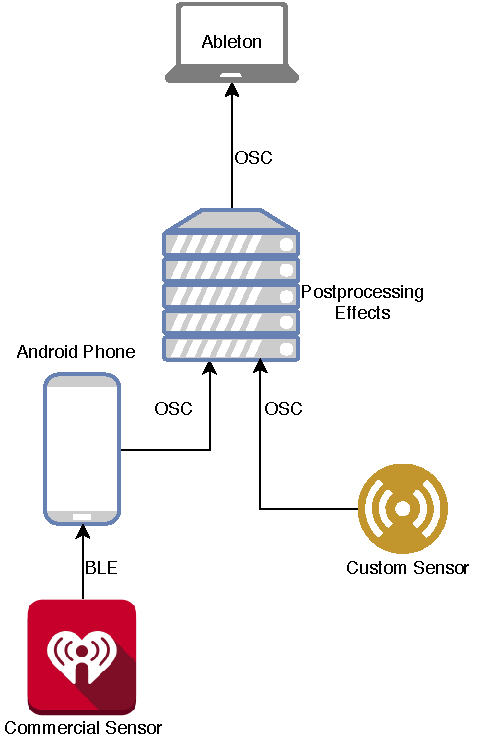
\includegraphics[width=0.9\marginparwidth]{figures/topology}
    \caption{Schematic view of the sensor and server setup}~\label{fig:setup}
  \end{minipage}
\end{marginfigure}

\begin{marginfigure}[-3pc]
  \begin{minipage}{\marginparwidth}
    \centering
    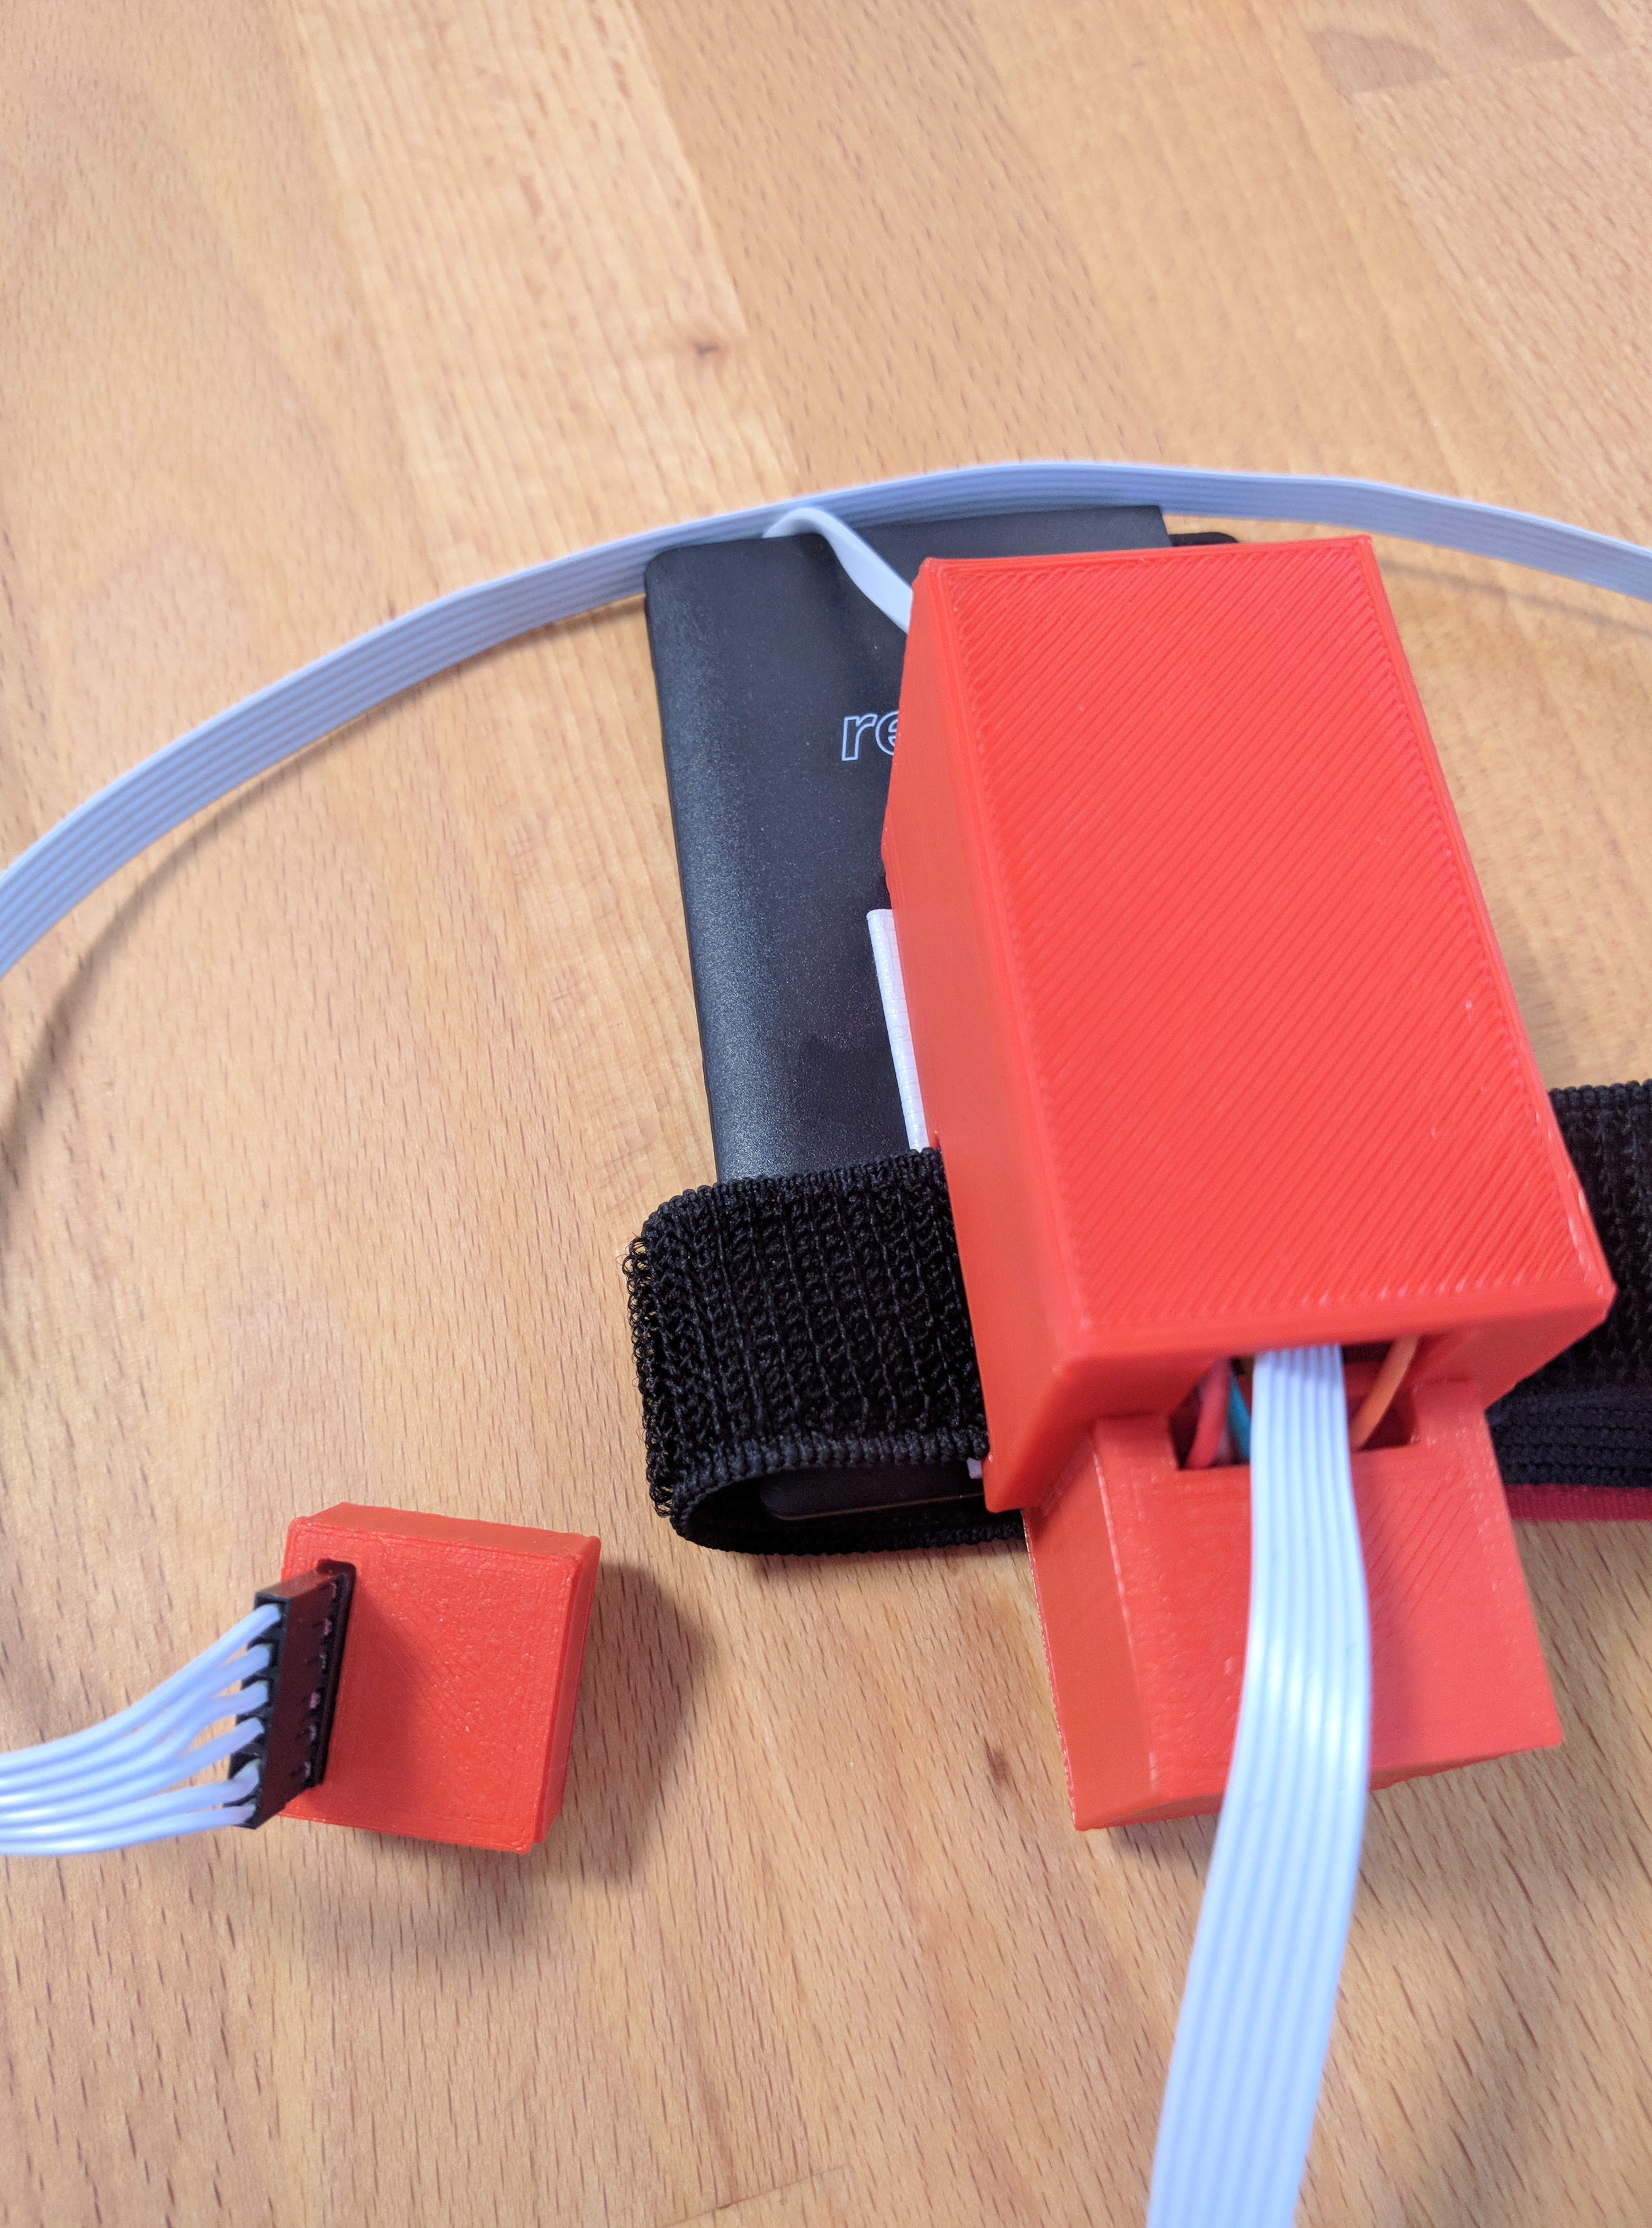
\includegraphics[width=0.9\marginparwidth]{figures/sensor}
    \caption{Custom sensor setup}~\label{fig:sensor}
  \end{minipage}
\end{marginfigure}

\subsection{custom}
The custom sensor setup is made up of a PPG sensor, a three-axis accelerometer and an ESP32 module. Power supply
is provided by a standard USB power bank. As heart rate sensor a BH1792GLC from Rohm Semiconductor is used.
This device drives green LEDs and stores the intensity of light reflected from human body in registers.[Datenblatt BH1792GLC]
These registers are read out via I2C by the ESP32 module every $20ms$. The power for the green LEDs has to
be adjusted depending on the position where the sensor is placed on human body. \\
Respiration rate is calculated on the server based on data of the accelerometer MMA8452Q of NXP Semiconductors.
The output data rate is preset to $50Hz$ and the registers of the accelerometer are read out via I2C as well.
The data is directly forwarded to the server by the ESP32 module using OSC over Wifi. The OSC message consists of a
header with information about type of data (heart rate or respiration rate) and a hard coded ID to distinguish
different custom sensor systems, as well as the data itself. \\
The proprietary casing for the sensors, ESP32 module and wiring was 3D-printed. The finished sensor can be seen
in figure~\ref{fig:sensor} and is attached to the upper arm.

\section{Results}

We have been able to extract both the heart rate and the respiration rate using a hardware setup that can be
worn easily on the body. Both values are accurate enough for the requirements of our goal, which has been
effect generation based on the gathered bio signals. However, only the heart rate yields a bandwidth of values
that is wide enough to be interesting for effects.

The respiration rate does only change in a window between 12 and 16 breaths per minute under normal conditions.
Furthermore, our implementation can only change its value in integer values, resulting in either a very small
effect range or sharp, abrupt changes in the effect. %TODO: signalprocessing: explain, peak counting...

While it might be feasible from a technical point of view to control elements of a performance using the respiration
rate of the performer, it is not feasible to do so from the performing point of view. Our method does not detect
sudden changes in the respiration, but calculates the average over a fixed time span. Hence it would be necessary
to keep the respiration rate at a significantly changed value over a prolonged time. This is very hard, we were
not able to achieve this while focussing only on this task. Doing it while performing on stage would be even harder.

The heart rate has a much wider span of values and can be used for various effects. In our own demonstration we used
it to change a sound effect based on the range of the value a single sensor provides or based on the gap or the average
between multiple sensors. Visually we logged the values of every connected sensor and generated graphs showing the
heart rate over time.

During our test runs two distinctive patterns emerged time and again: First, the heart rate of a performer
drops significantly after starting the performance. Second, regarding a listener, the heart rate slowly rises
in ``suspension building'' sections and drops sharply on their conclusion. This could be used to highlight
breaks in a performance using effects based on the heart rate.

\balance{} 

\bibliographystyle{SIGCHI-Reference-Format}
\bibliography{references}

\end{document}

%%% Local Variables:
%%% mode: latex
%%% TeX-master: t
%%% End:
